% Modelo de slides para projetos de disciplinas do Abel
\documentclass[10pt]{beamer}

\usetheme[progressbar=frametitle]{metropolis}
\usepackage{appendixnumberbeamer}
%\usepackage[numbers,sort&compress]{natbib}
%\bibliographystyle{plainnat}
%\usepackage[numbers]{natbib}
%\usepackage[numbers,round]{natbib}
\usepackage{booktabs}
\usepackage[scale=2]{ccicons}
\usepackage{xspace}
\usepackage{natbib}
\newcommand{\themename}{\textbf{\textsc{metropolis}}\xspace}
\newcommand\Fontvi{\fontsize{6}{7.2}\selectfont}
\newcommand\Wider[2][5em]{%
\makebox[\linewidth][c]{%
  \begin{minipage}{\dimexpr\textwidth+#1\relax}
  \raggedright#2
  \end{minipage}%
  }%
}
\title{Reinforcement Learning - Continuous Cartpole}
% \subtitle{Subtítulo}
% \date{\today}
\date{}
\author{Aron Distelzweig}
\institute{Project}
% \titlegraphic{\hfill\includegraphics[height=1.5cm]{logo.pdf}}

\begin{document}
\setbeamercolor{background canvas}{bg=white!20}
\maketitle

\begin{frame}[fragile]{Approach}
\setbeamertemplate{itemize items}[ball]
\begin{itemize}
  \item Actor Critic method because of continuous action and state space
  \item Reward function: The smaller the angle, the higher the reward
  \item First approach: Deep Deterministic Policy Gradient (DDPG)
  \item DDPG shows unstable performance
  \item Turn DDPG into TD3 by adding the following three adjustments
  \begin{itemize}
  \item Clipped Double Q-Learning
  \item Delayed Policy Updates
  \item Target-policy smoothing
  \end{itemize}
\end{itemize}
\end{frame}

\begin{frame}[fragile]{Results - TD3}
\setbeamertemplate{itemize items}[ball]
  \begin{figure}
   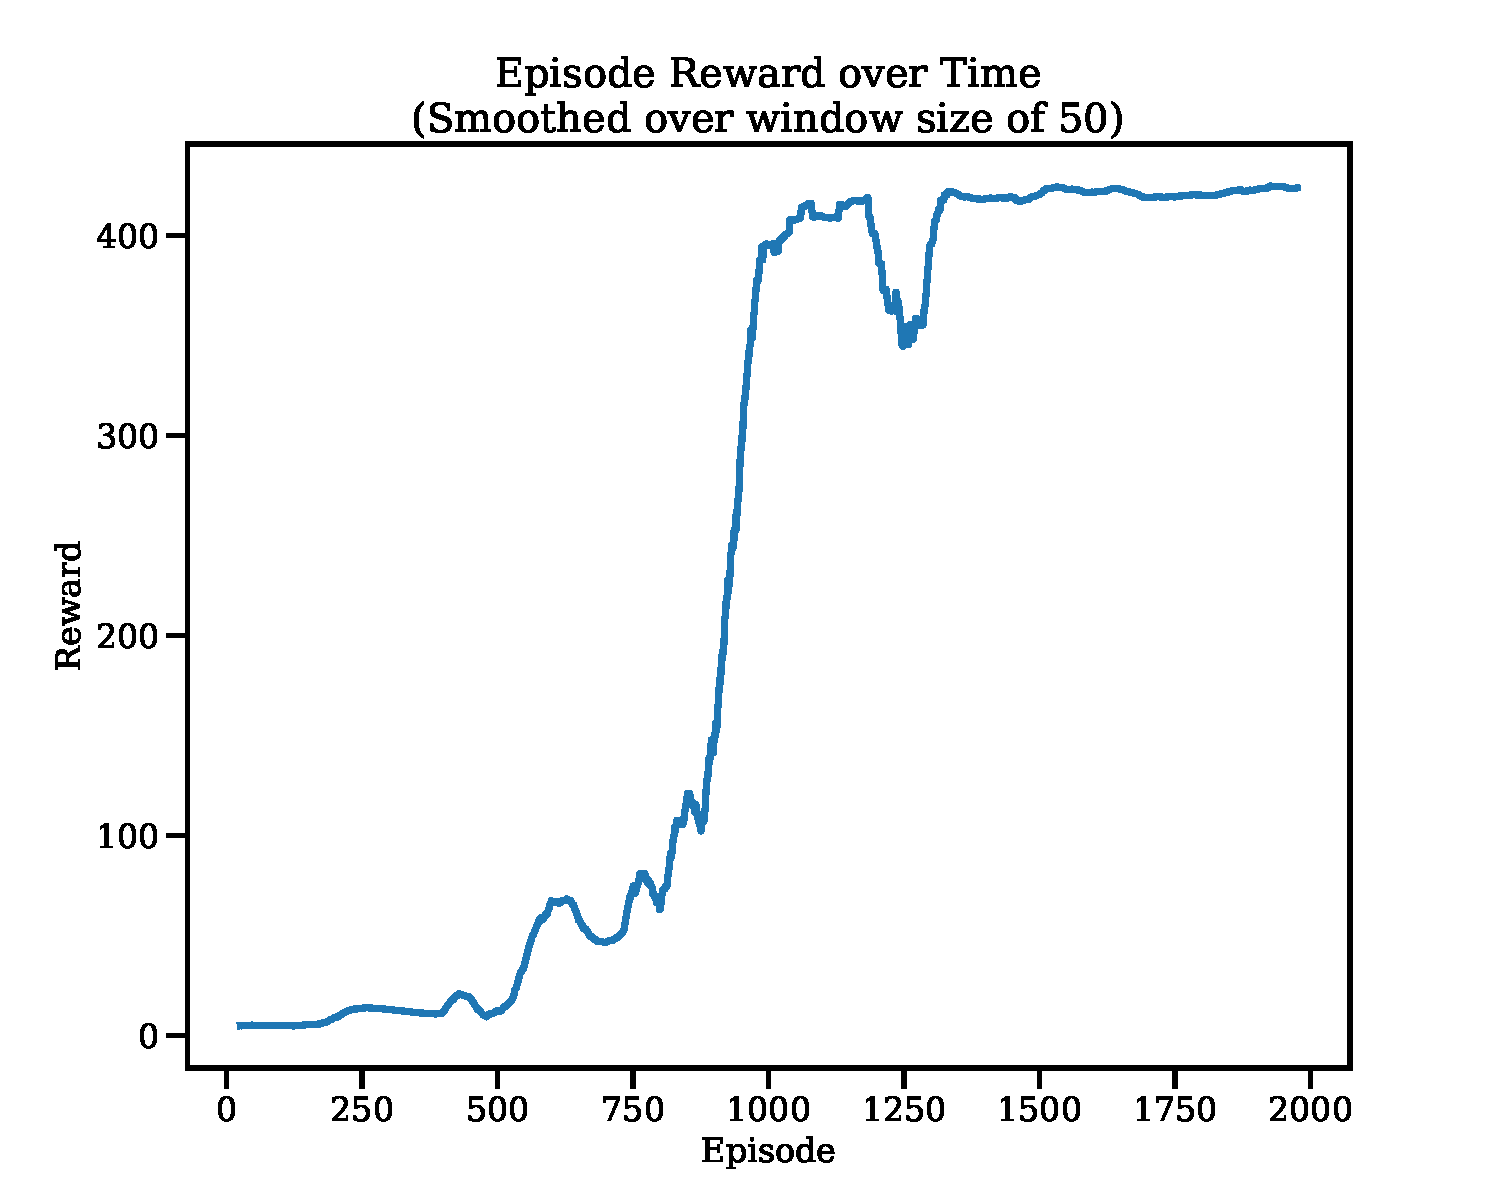
\includegraphics[scale=0.3]{../results/td3_res_episode_reward.pdf}
  \end{figure}
\end{frame}

\begin{frame}[fragile]{Results - TD3}
\setbeamertemplate{itemize items}[ball]
\begin{figure}[!htb]
\minipage{0.45\textwidth}
  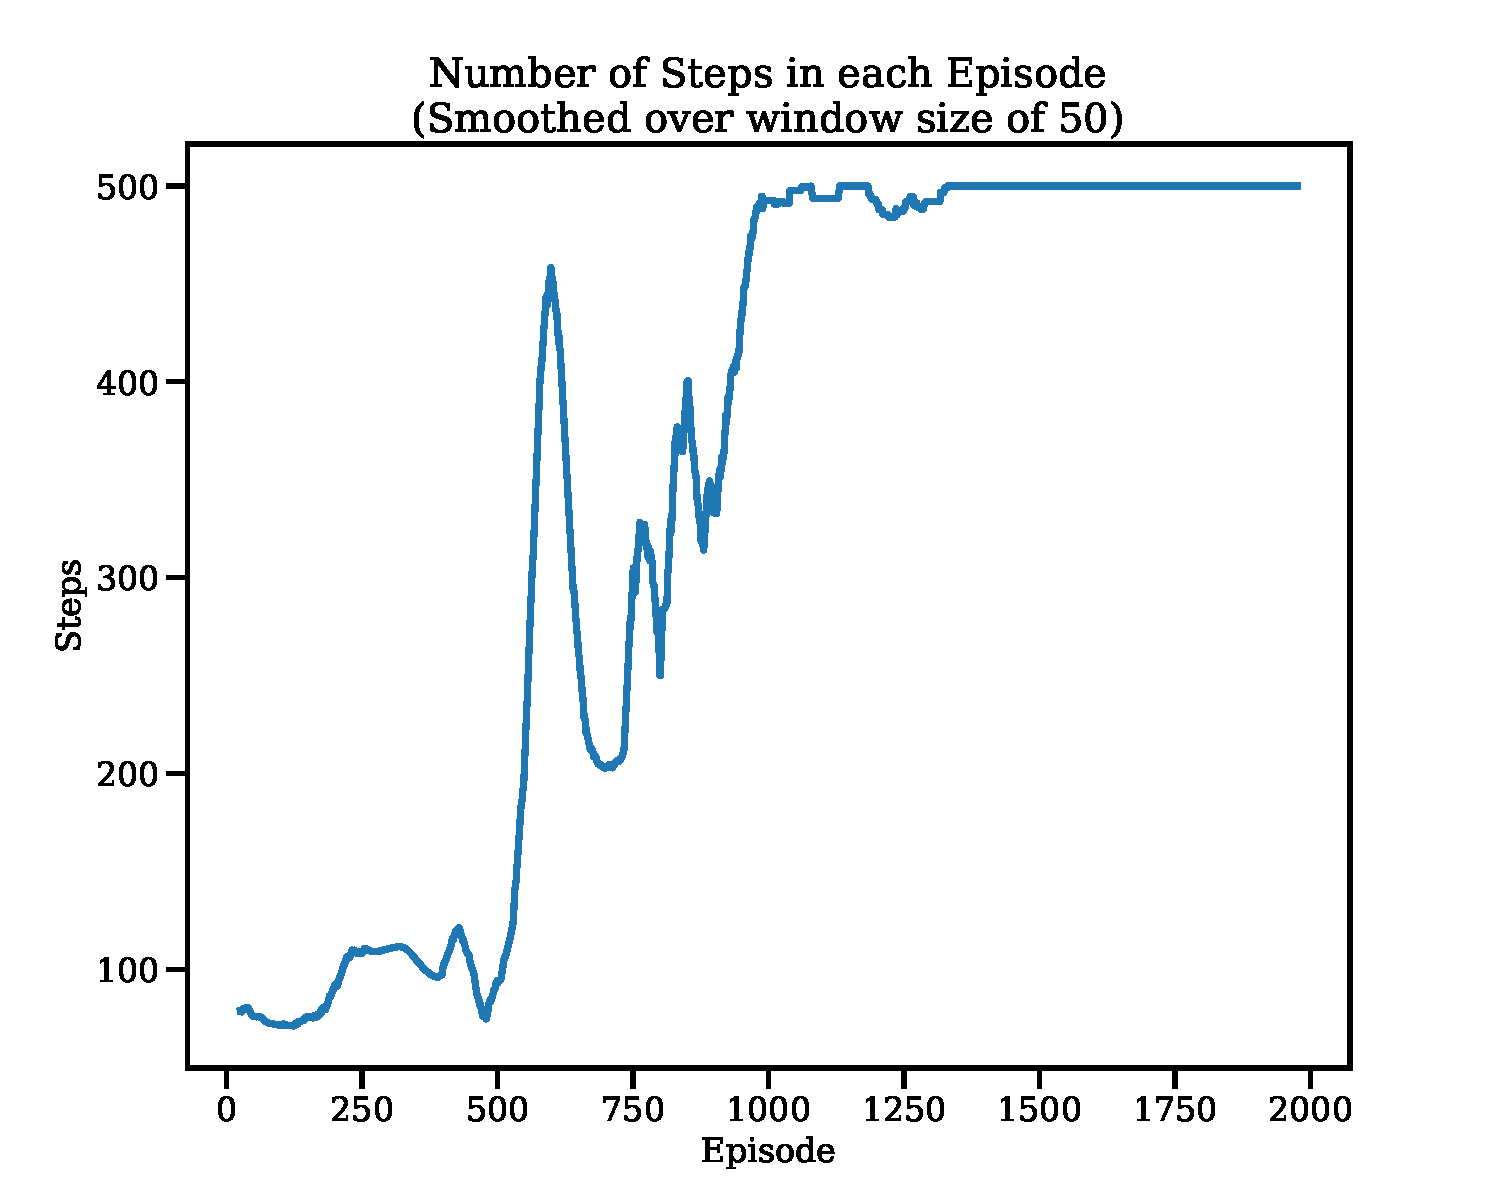
\includegraphics[width=\linewidth]{../results/td3_res_episode_steps.pdf}
\endminipage\hfill
\minipage{0.45\textwidth}
  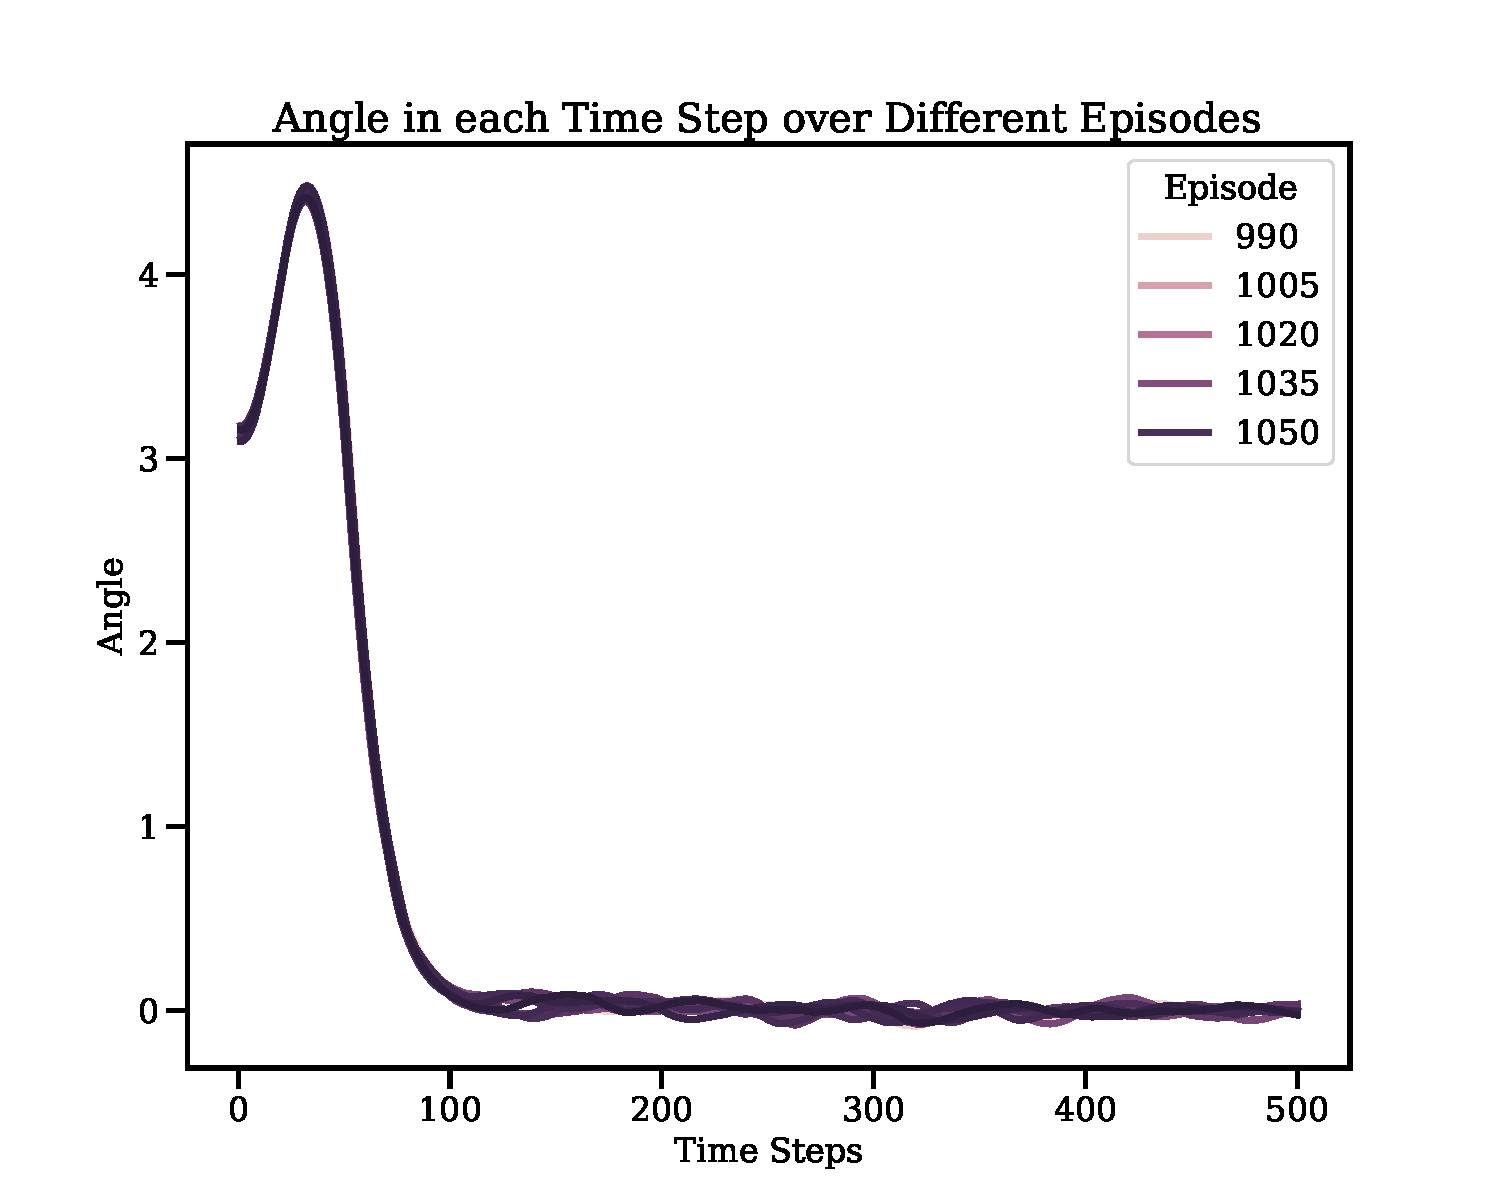
\includegraphics[width=\linewidth]{../results/td3_res_Angle.pdf}
\endminipage\hfill
\minipage{0.45\textwidth}
  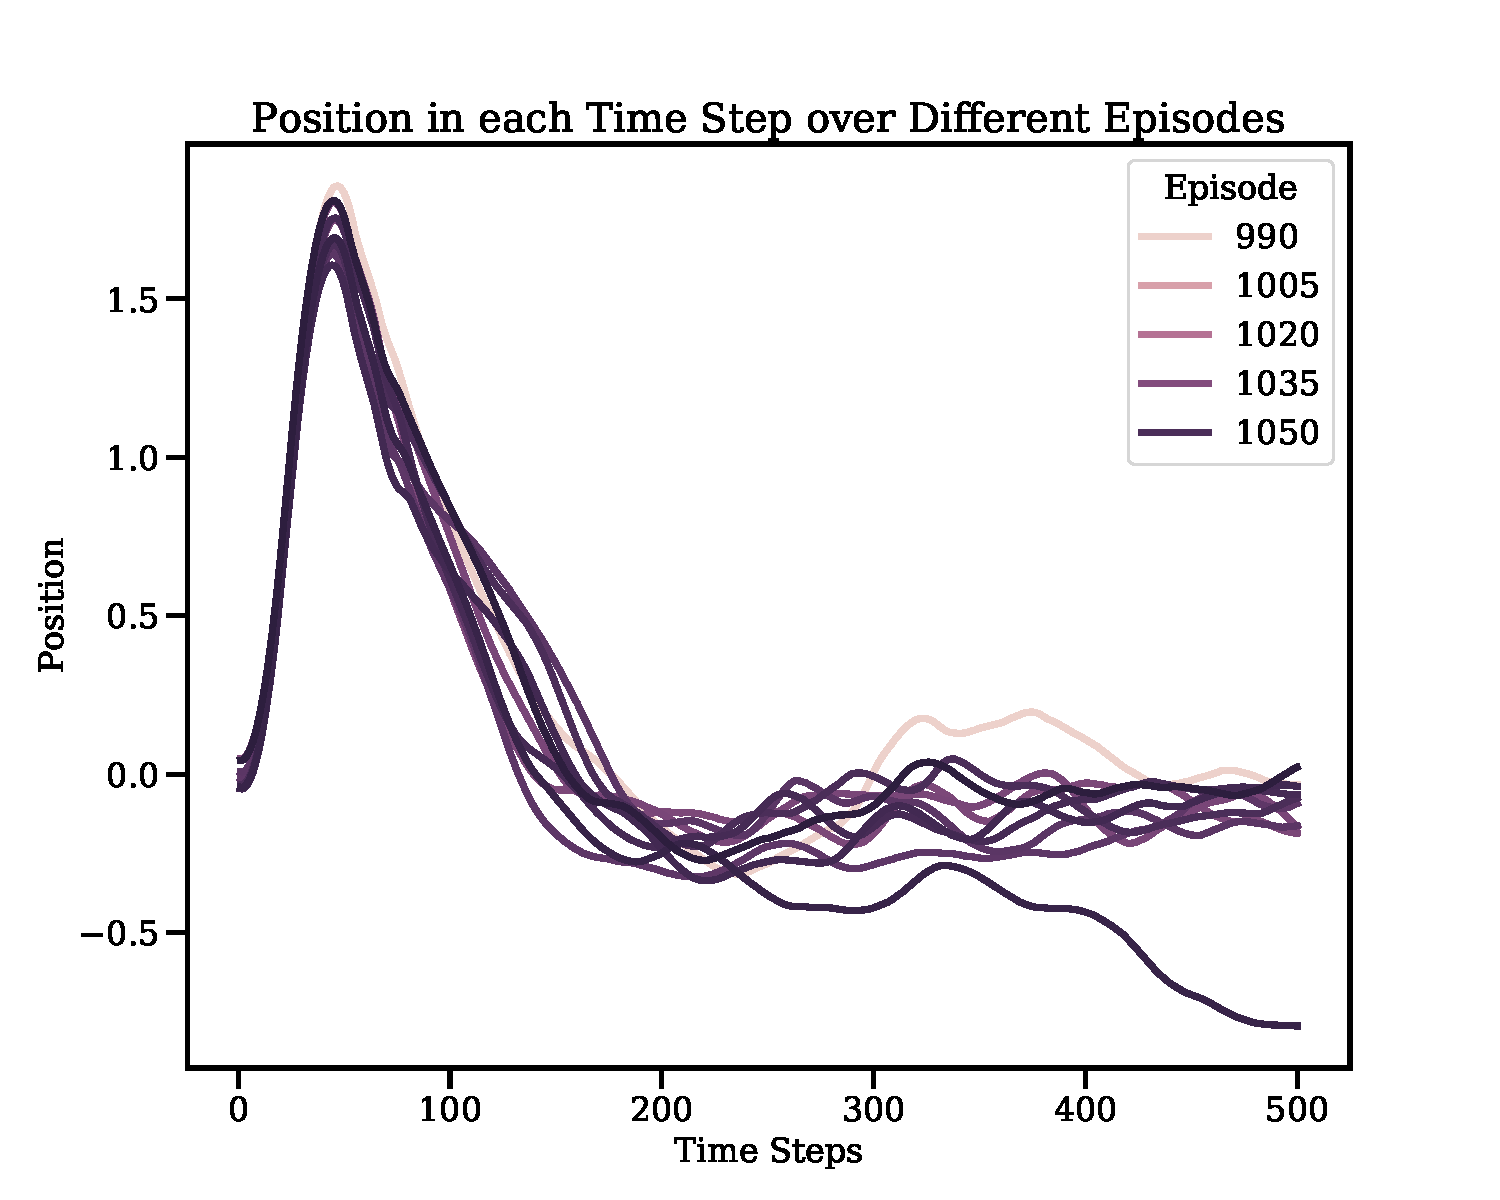
\includegraphics[width=\linewidth]{../results/td3_res_Position.pdf}
\endminipage\hfill
\minipage{0.45\textwidth}
  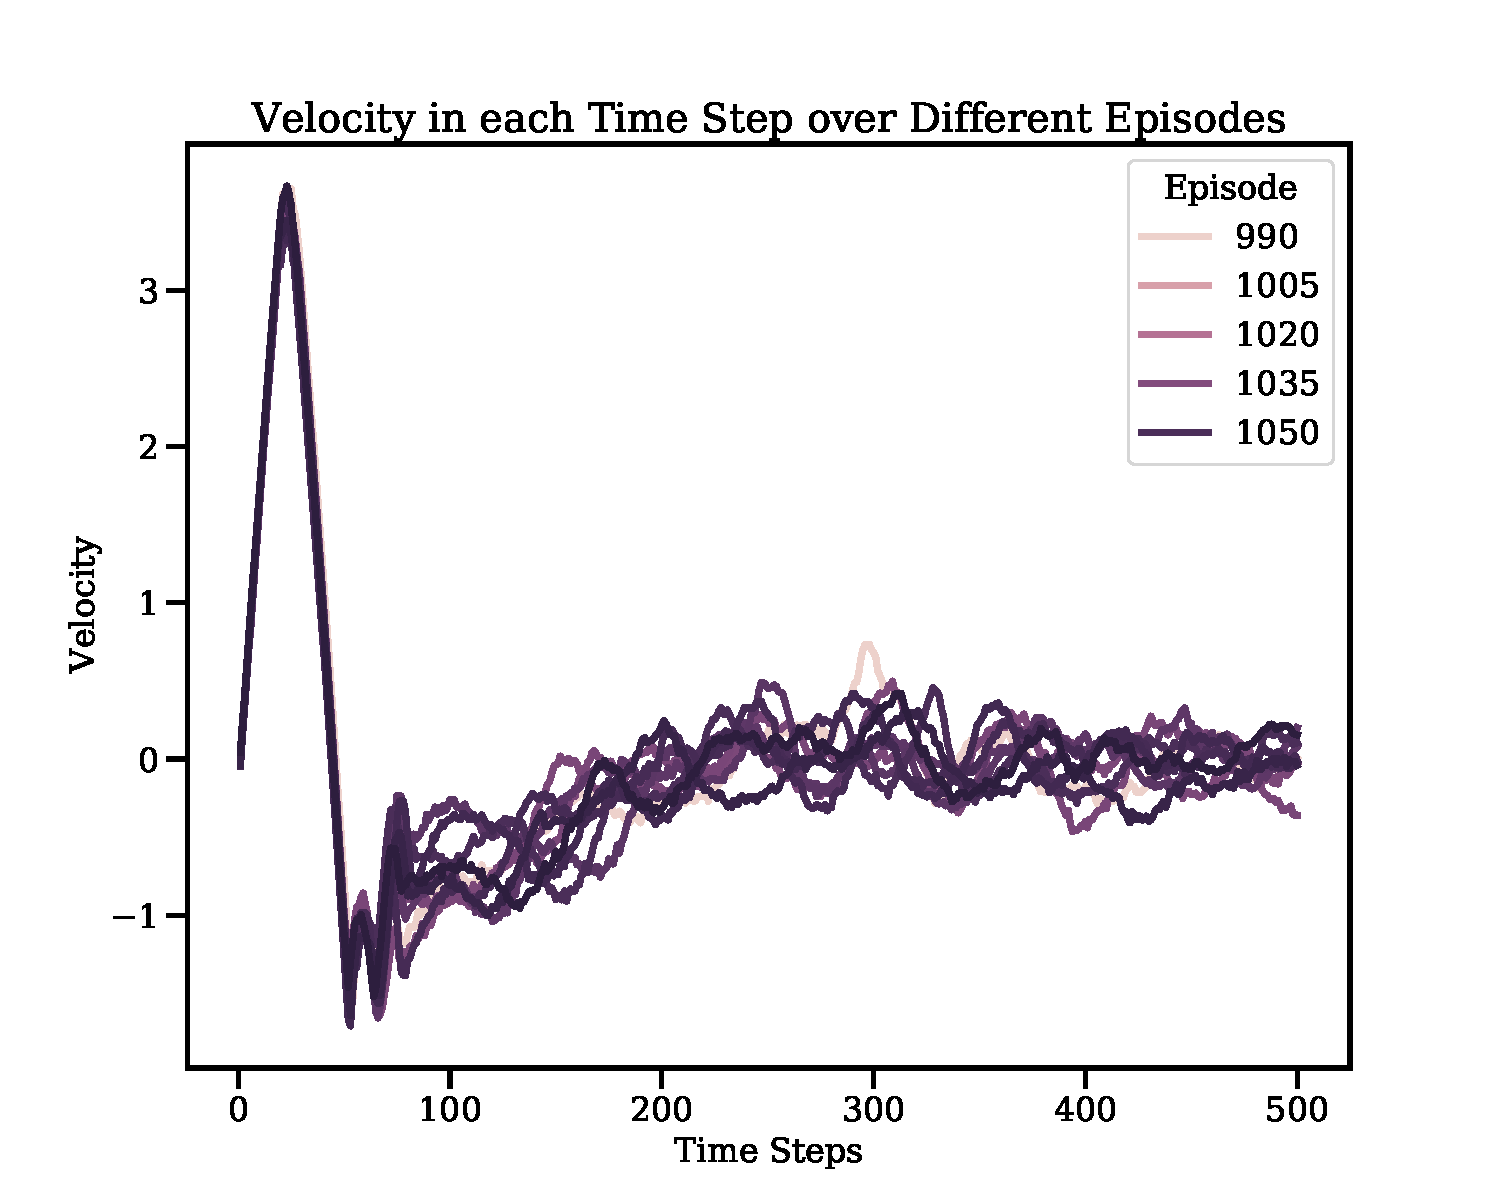
\includegraphics[width=\linewidth]{../results/td3_res_Velocity.pdf}
\endminipage\hfill
\end{figure}

\end{frame}



\begin{frame}[fragile]{Results - DDPG}
\setbeamertemplate{itemize items}[ball]
\begin{figure}[!htb]
\minipage{0.45\textwidth}
  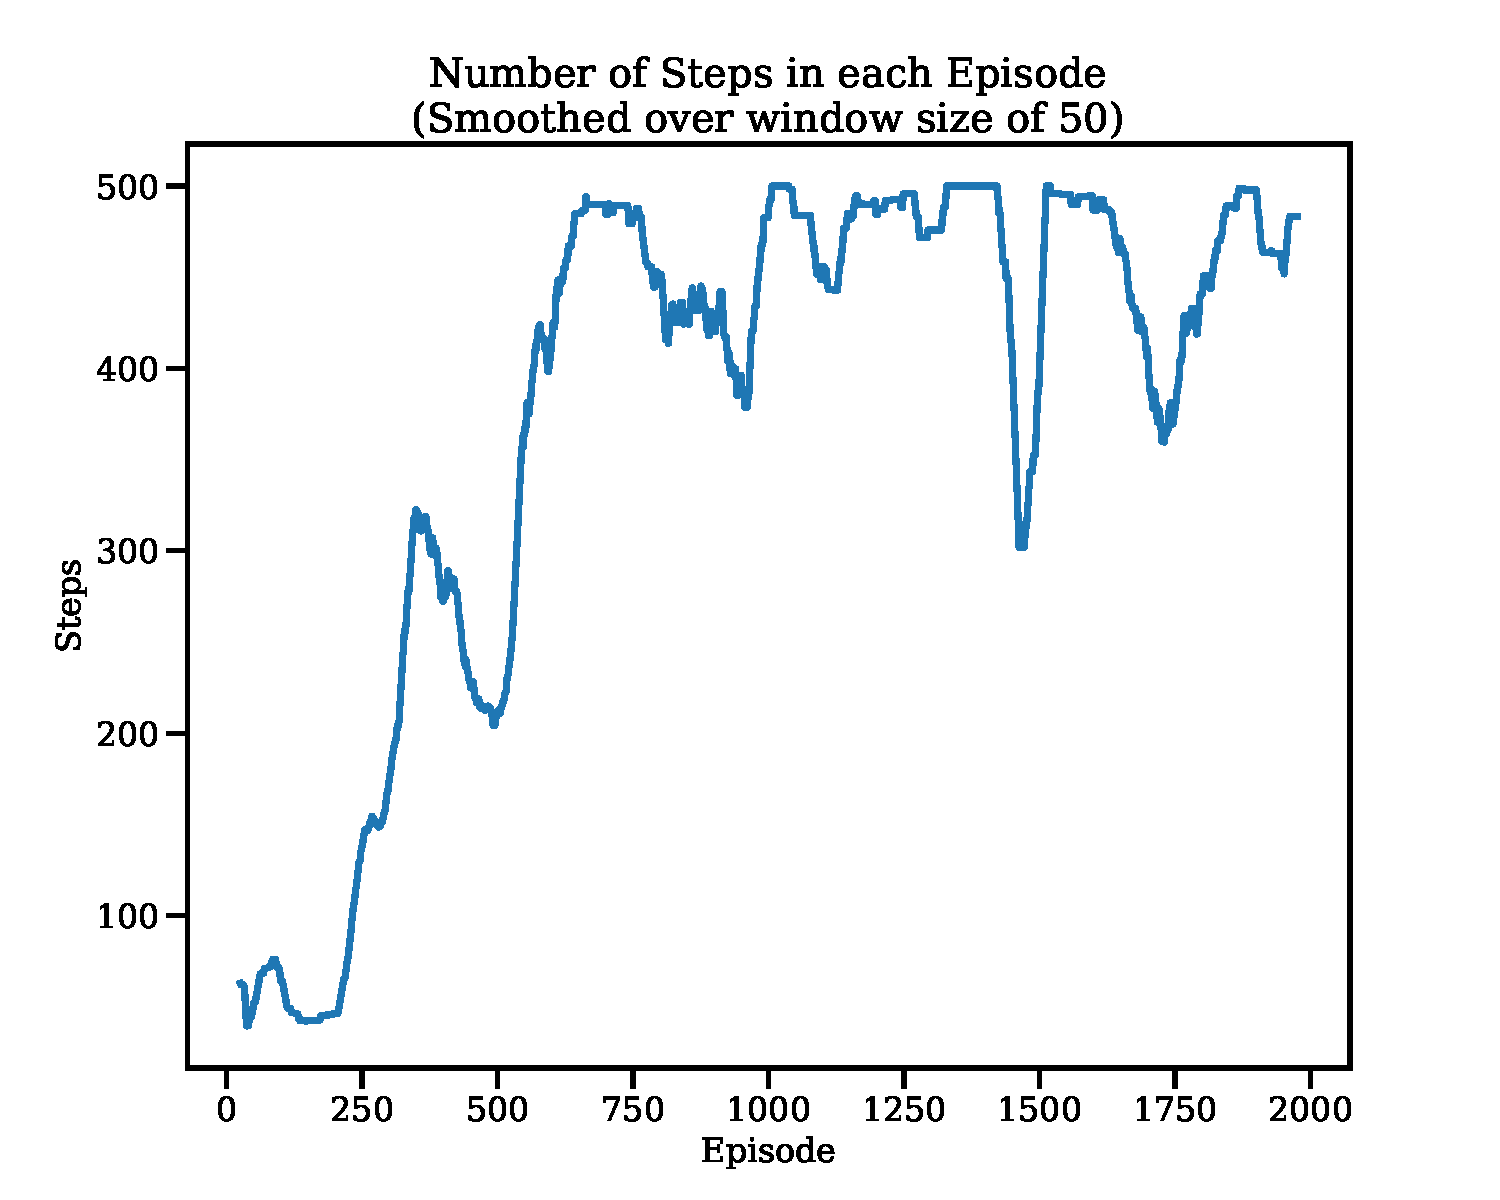
\includegraphics[width=\linewidth]{../results/ddpg_res_episode_steps.pdf}
\endminipage\hfill
\minipage{0.45\textwidth}
  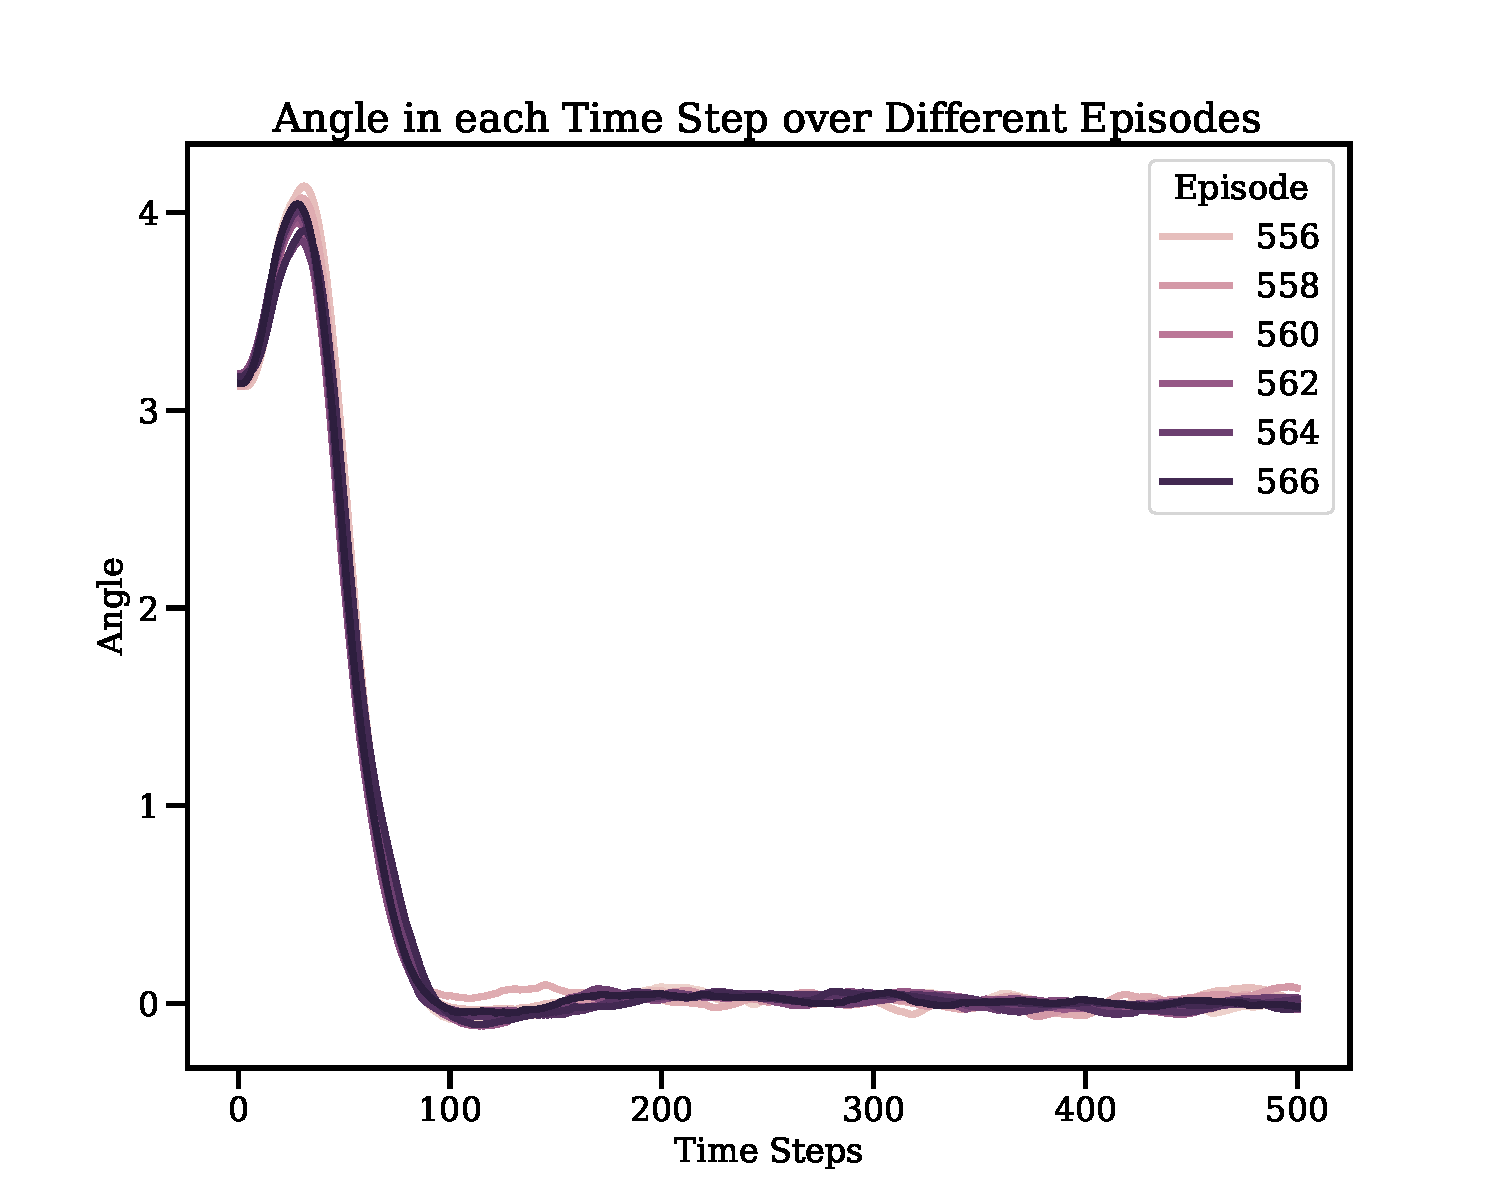
\includegraphics[width=\linewidth]{../results/ddpg_res_Angle.pdf}
\endminipage\hfill
\minipage{0.45\textwidth}
  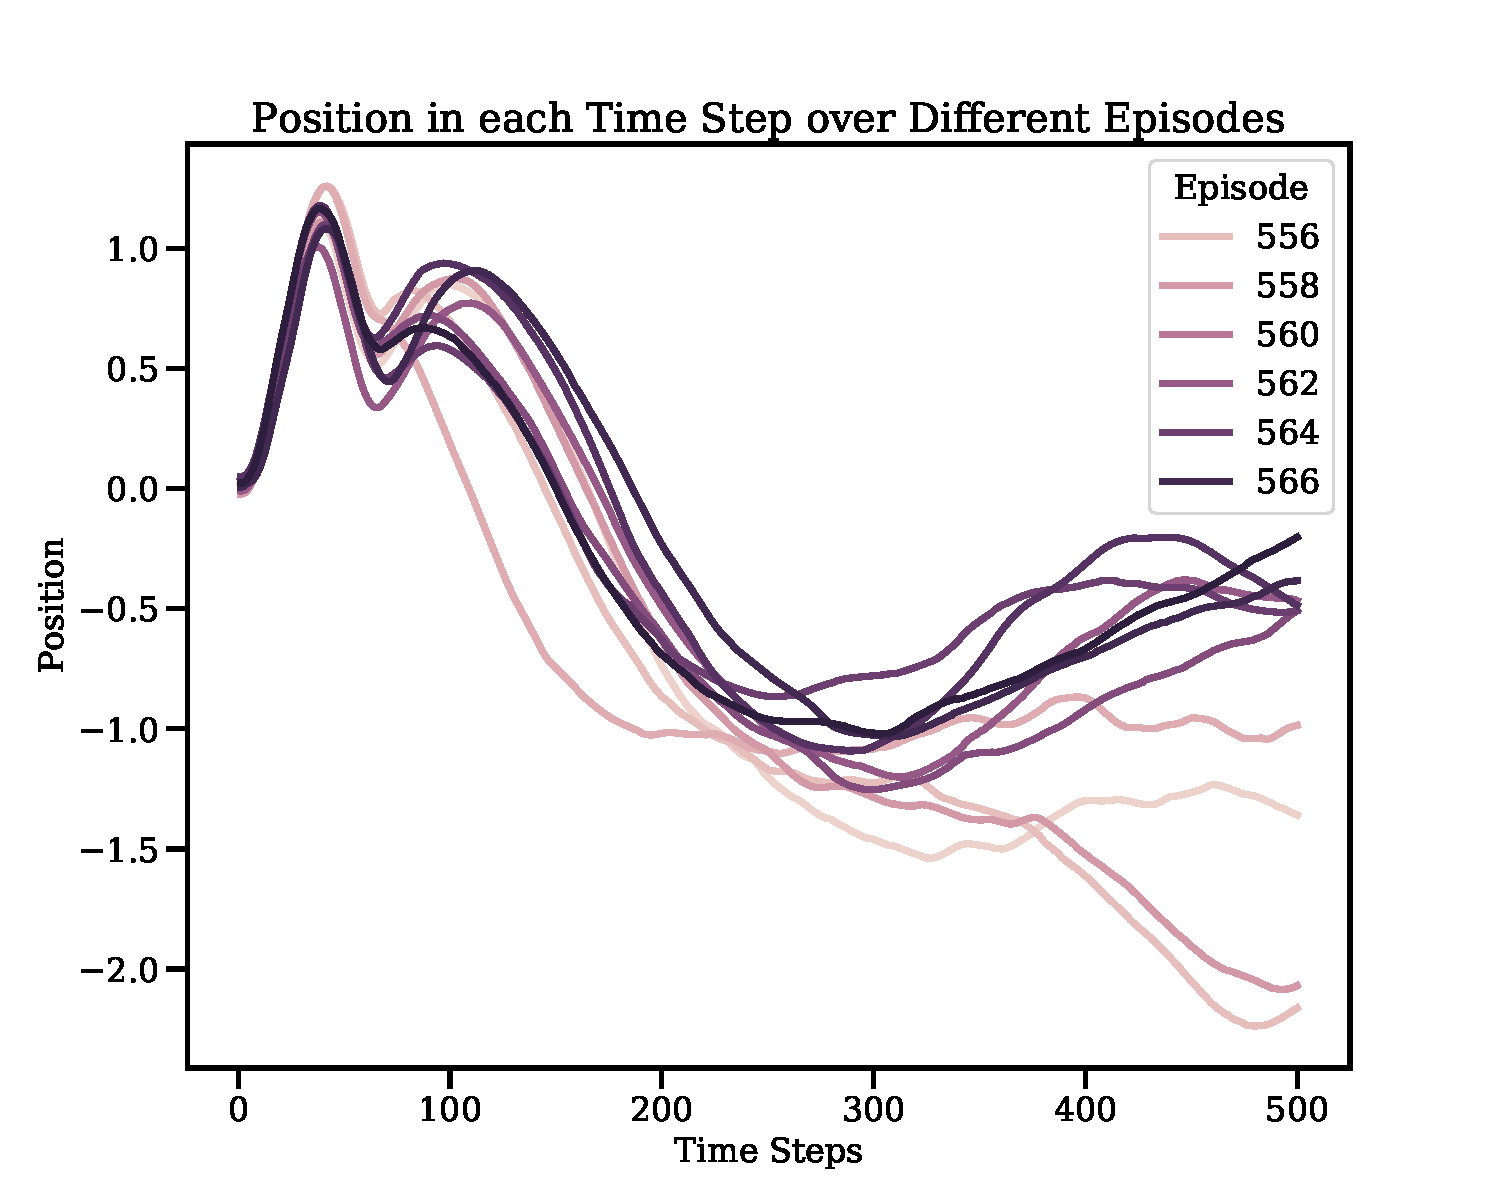
\includegraphics[width=\linewidth]{../results/ddpg_res_Position.pdf}
\endminipage\hfill
\minipage{0.45\textwidth}
  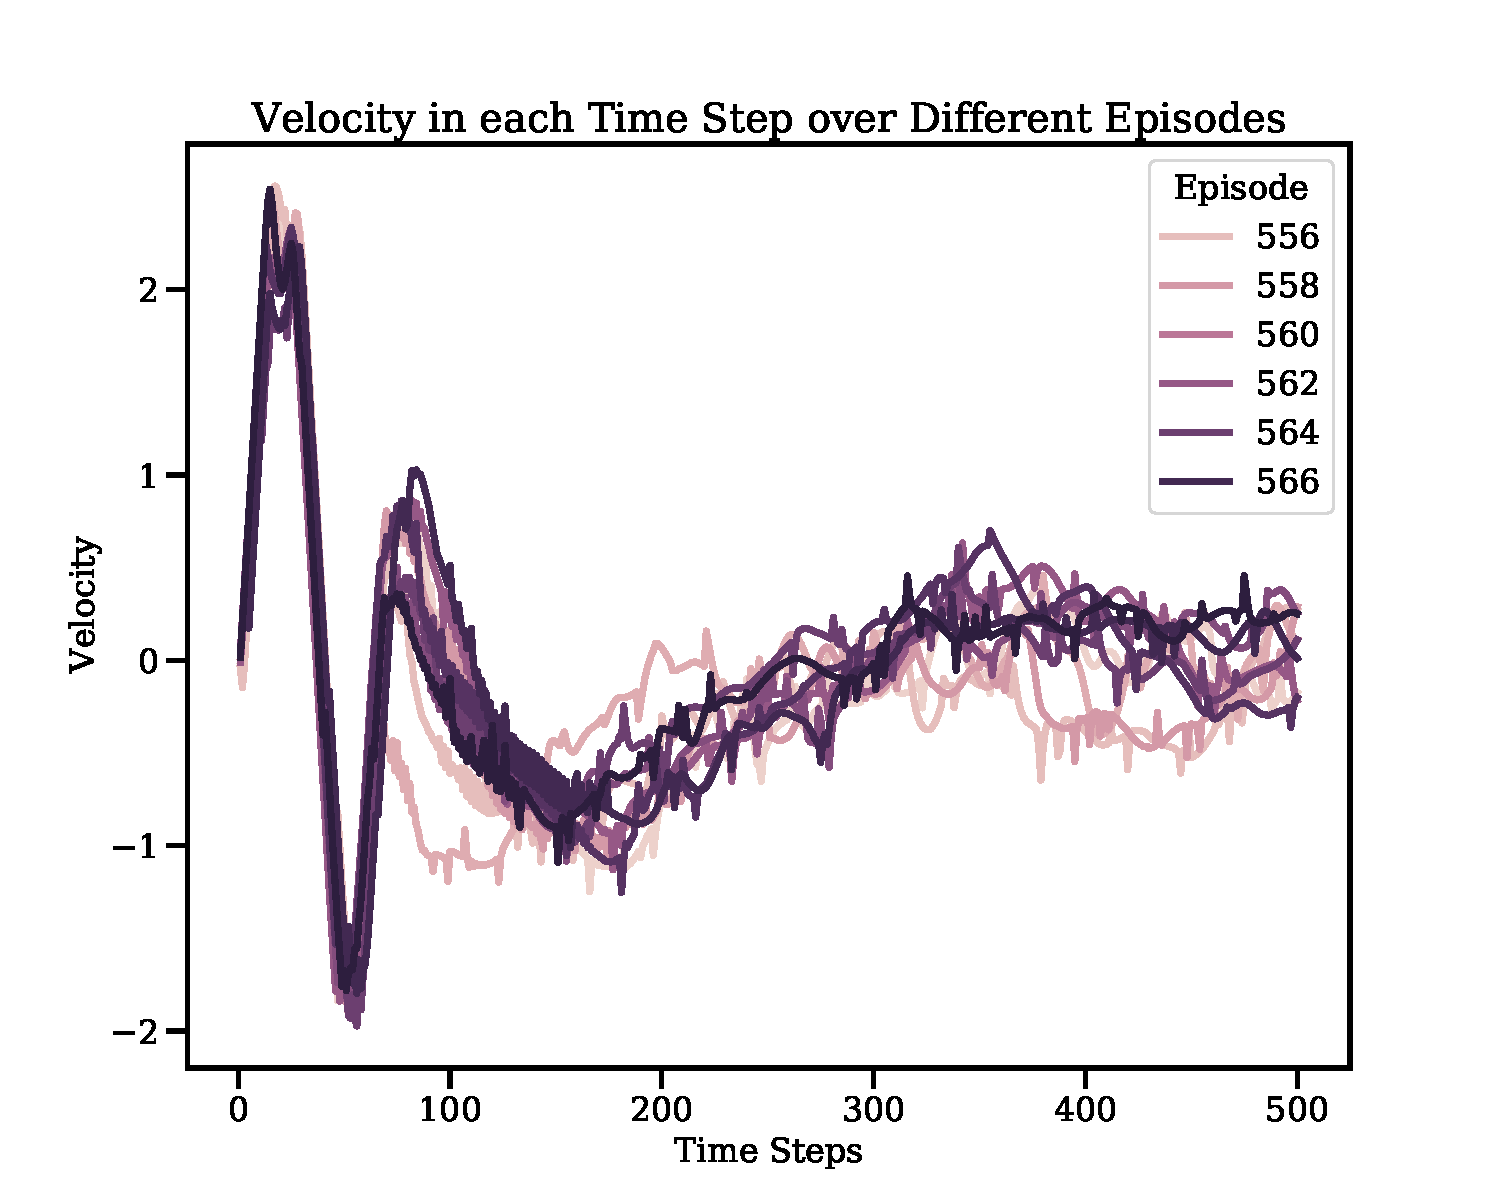
\includegraphics[width=\linewidth]{../results/ddpg_res_Velocity.pdf}
\endminipage\hfill
\end{figure}
\end{frame}


\begin{frame}[fragile]{TD3}
\setbeamertemplate{itemize items}[ball]
  \begin{figure}
   \includegraphics[scale=0.15]{../../../td3.png}
  \end{figure}
\end{frame}

\end{document}
